\chapter{Leader-Follower Control Mode}
\label{ch:LFCM}
The leader-follower control problem can roughly be defined as a regulation control problem where the follower must maintain a specified formation determined by a rectangular longitudinal and lateral offset defined in the leader's body-fixed, cartesian frame. This idea is illustrated in Fig. \ref{fig:Leader_Follower_Rectangular_Diagram}.
\begin{figure}[b]
\begin{subfigure}{0.525\textwidth}
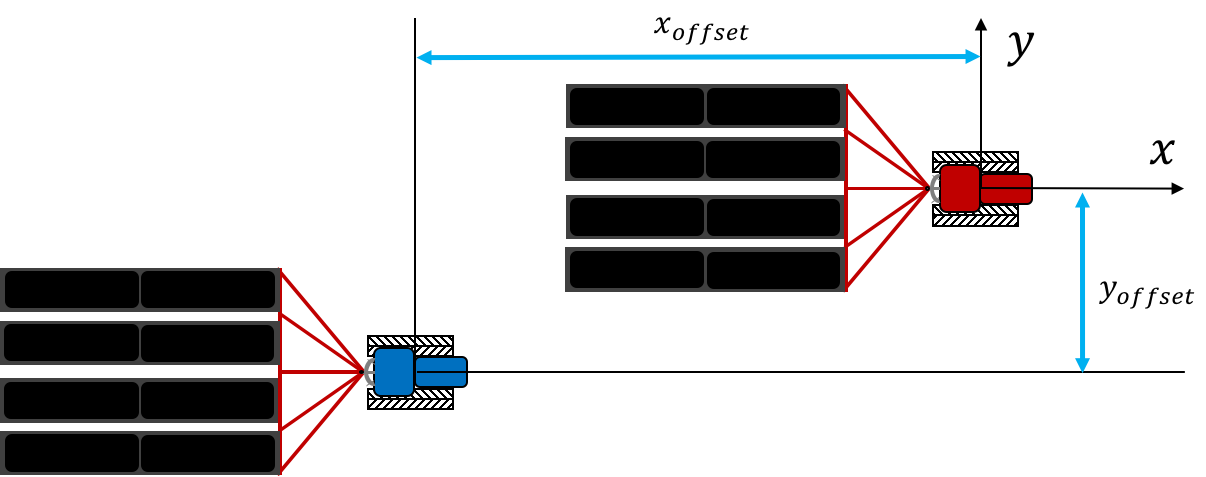
\includegraphics[height = 2.75 cm, keepaspectratio]{Leader_Follower_Rectangular_Diagram}
\caption{}
\label{fig:Leader_Follower_Rectangular_Diagram}
\end{subfigure}
\begin{subfigure}{0.525\textwidth}
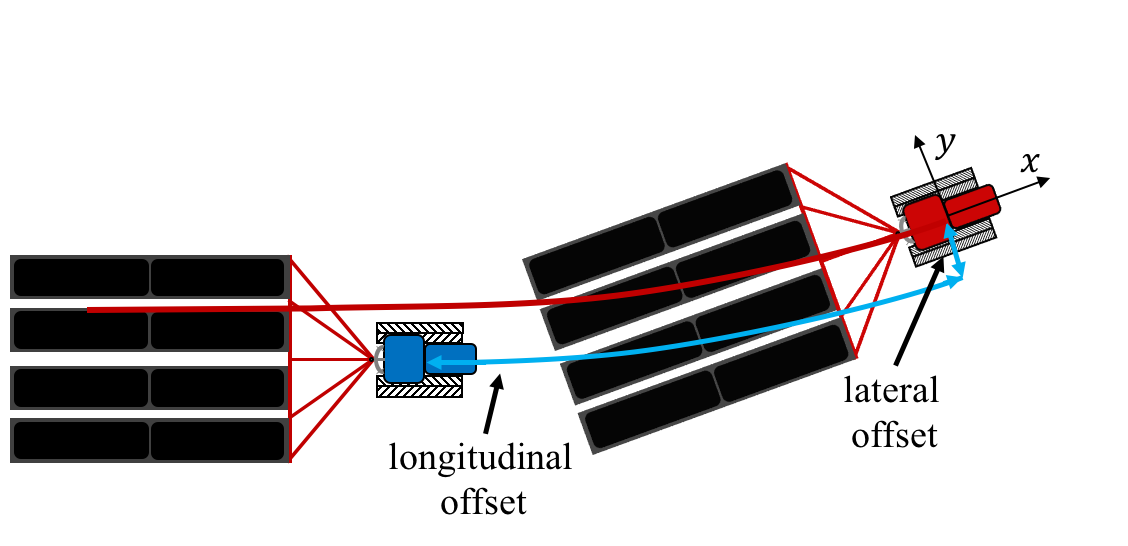
\includegraphics[height = 3.4cm, keepaspectratio]{Leader_Follower_Curvilinear_Diagram}
\caption{}
\label{fig:Leader_Follower_Curvilinear_Diagram}
\end{subfigure}
\caption{(a) Rectangular coordinate leader follower formation.  (b) Flexible, curivilinear coordinate leader follower formation.  (a \& b) Leader tractors are colored red, follower tractors are colored blue.}
\label{fig:Leader_Follower_Concept}
\end{figure}
This requirement is quite strict and recent developments have proposed regulation of a flexible curvilinear formation shown in Fig. \ref{fig:Leader_Follower_Curvilinear_Diagram} \cite{barfoot2004motion}. Here the follower follows a reference trajectory that is generated as a lateral offset from the leader's nominal trajectory where time parameterized velocities and yaw rates are computed via kinematic constraints in curvilinear coordinates \cite{barfoot2004motion}. However, the leaders in this study are also unmanned so these nominal trajectories are absent from noise and disturbances since they are computed via a higher level planner. This approach is not readily applicable to systems with manned leader's in the loop with noisy velocity and yaw rate reference signals. Low \cite{low2015flexible, low2014flexible} adapts the method presented by Barfoot \cite{barfoot2004motion} for a SUV manned leader by sampling the leader's trajectory at 20 Hz and generating a tracked vehicle follower reference trajectory at the sampled points. A continuous trajectory for velocity and yaw rate is then approximated using linear interpolation and followed using low level velocity and yaw rate controllers built into the tracked vehicle platform.

The method presented here uses the idea of maintaining a flexible formation but in a different way than the works previously discussed. These previous studies have implemented methods on two wheeled robots and a much lighter tracked vehicle under no drawbar load. There is also an implicit assumption that leader vehicle trajectories produce reference follower trajectories that are dynamically feasible. This may not always be the case for human-in-the-loop systems as proposed for SPT where manned leaders will be operating at $\sim$100\% engine load in the highest gear ratio possible to minimize traverse times. This idea can be visualized by refering back to Fig. \ref{fig:Leader_Follower_Curvilinear_Diagram}. Here, if the follower tractor follows a trajectory that is a perfect offset of the leader, this trajectory requires a larger arc length to be traveled in the same amount of time. If there is no extra engine torque capacity, this trajectory will not be feasible. Therefore, the idea of maintaining a flexible formation is extended beyond curvilinear coordinates by using a way point following strategy. Here, way points are used as a path guide instead of providing a strict reference trajectory in combination with low level controllers for velocity and heading regulation. 
\import{Chapter5/}{Way_Point_Following}
\import{Chapter5/}{Velocity_and_Heading_Controllers}
\import{Chapter5/}{Simulation_Results}
\import{Chapter5/}{Formation_Changes}